%------------------------------------------------------------------------------
% Tema 6. Hemoglobina i ferro
%------------------------------------------------------------------------------
\section{Hemoglobina i ferro}

\subsection{La hemoglobina}
La hemoglobina és una proteïna globular que dona la coloració vermella
de la sang. Responsable del transport de \ch{O2}. Té un pes de  64,45
kDa.

Els nivells normals són de 16g/100 mL en homes i de 14g/100 mL en les dones.

Un home de 70 kg té 900 g d'hemoglobina. El bescanvi d'hemoglobina és
de 0,3 g/h (sintetitzats i destruïts).

Classificació de les malalties relacionades amb la hemoglobina:
\begin{itemize}
\item Reaccions de l'hemoglobina
  \begin{itemize}
  \item Metahemoglobinèmia hereditària
  \end{itemize}

\item Síntesi de la globina
  \begin{itemize}
  \item Hemoglobinopaties estructurals
    \begin{itemize}
    \item Anèmies drepanocítiques 
    \item Metahemoglobinèmia congènita
    \item Eritrocitosis (alterada afinitat per O2)
    \end{itemize}
  \item Talassèmies (hemoglobines alterades)
    \begin{itemize}
    \item  $\alpha$-talassèmies
    \item $\beta$-talassèmies
    \end{itemize}
  \end{itemize}

\item Síntesi i degradació del grup hemo
  \begin{itemize}
  \item Porfiries agudes
    \begin{itemize}
    \item Porfíria aguda intermitent 
    \item Coproporfíria hereditària
    \item Porfíria variegata
   \end{itemize}
  \item Porfíries no agudes
    \begin{itemize}
    \item Porfíria eritrohepàtica (eritropoiètica) 
    \item Porfíria eritropoiètica congènita
    \item Porfíria congènita (Intoxicació per plom)
    \end{itemize}
  \end{itemize}

\item Alteracions del metabolisme del ferro
  \begin{itemize}
  \item Anèmia ferropènica (manca de ferro)
    \begin{itemize}
    \item Pèrdua crònica de sang
    \item Ingesta inadequada de ferro
    \end{itemize}
  \item Anèmia sideroblàstica (mala utilització del ferro)
  \item Hemocromatosis (sobrecàrrega de ferro)
  \end{itemize}
\end{itemize}

\subsubsection{Estructura}
Hi ha 6 tipus de globines, que en la seva combinatòria generen els
diferents tipus d'hemoglobina que trobem en humans. Aquests tipus són:
$\alpha$, $\beta$, $\gamma$, $\delta$, $\epsilon$, $\zeta$.

La hemoglobina és un heterotetràmer $\alpha_2\beta_2$ en adults. Presenta
cooperativitat amb l'oxigen. També té al·losterisme amb el
2,3-difosfoglicerat, un intermediari de la glicòlisi que només es
troba en eritròcits. Això facilita l'alliberació d'oxigen als
teixits.

Es sintetitza als reticulòcits (eritròcits immadurs).

La hemoglobina presenta diferents subunitats segons l'estadi de
desenvolupament de l'individu:
\begin{itemize}
\item Adult:
  \begin{itemize}
  \item Hemoglobina A1 ($\alpha_2\beta_2$)
  \item Hemoglobina A2 ($\alpha_2\delta_2$)
  \end{itemize}

\item Fetal: Cadenes $\alpha_2\gamma_2$

\item Embrió:
  \begin{itemize}
  \item Grower I: $\zeta_2\epsilon_2$
  \item Grower II: $\alpha_2\epsilon_2$
  \item Portland: $\zeta_2\gamma_2$
  \end{itemize}
\end{itemize}

Hi ha 2 loci d' $\alpha$-globina al cromosoma 16 i un locus de $\beta$-globina
al cromosoma 11.

\subsection{Trastorns deguts a reaccions de l'hemoglobina}
La carboxihemoglobina presenta menys afinitat per l'hemoglobina.

\begin{figure}[H]
  \centering
  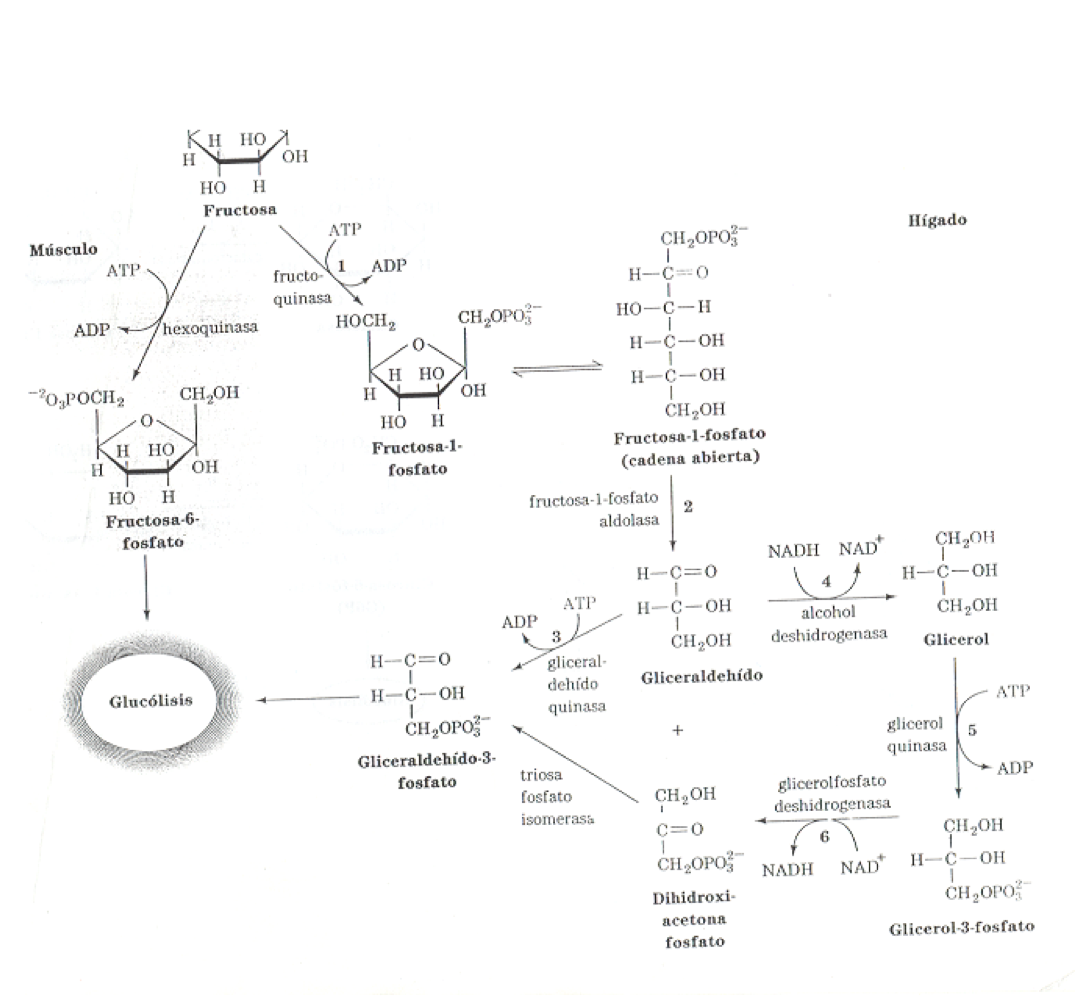
\includegraphics[width=0.5\textwidth]{fig5}
\end{figure}

Molt fàrmacs o agents oxidants poden provocar la formació de
metahemoglobina (amb \ch{Fe3+}), que mitjançant la NADH-metahemoglobina
reductasa la torna a reduir.

\begin{figure}[H]
  \centering
  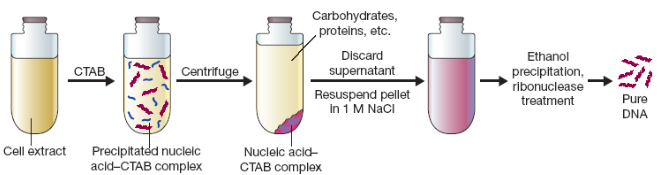
\includegraphics[width=0.5\textwidth]{fig6}
\end{figure}

La metahemoglobinèmia hereditària és una deficiència en NADH-metahemoglobina
reductasa. El Fe del hemo s'oxida en 25 \% a \ch{Fe3+} Es manifesta amb
cianosi (coloració fosca a la pell). Es tracta amb fàrmacs que
redueixin lametahemoglobina. És una malaltia
molt greu.

\subsection{Trastorns a la síntesi de la globina}
\subsubsection{Hemoglobinopaties estructurals}
Les mutacions perjudicials desapareixen, però les altres poden sobreviure
(els heterozigots resisteixen més que els homozigots). Algunes
mutacions són inòcues.

\paragraph{Hemoglobina S. Anèmia drepanocítica} \hfill \\
Es dóna un canvi d'aminoàcid Glu->Val a la cadena beta. És insoluble a baixes pressions
de \ch{O2}. Els glòbuls vermells presenten una morfologia
falciforme. Quan està desoxigenada, la hemoglobina es polimeritza i es
deformen els eritròcits. Els heterozigots  presenten poques vegades símptomes greus

Es va originar a Africa i confereix resistència a la malària. La
presenten un 40 \% de la població africana i un 10\% dels negres
americans.

La Hb pot polimeritzar formant fibres de 3000 \AA{}. Hi ha cicles
successius de forma de falç i normal. La forma de falç es trenca als
capil·lars per falta de flexibilitat. L'anèmia s'agreuja amb oxidants.

Altes concentracions d'HbS d'afinitat baixa per \ch{O2} no donen cap
problema fins l'administració d'un agent oxidant.

L'anèmia és menys severa si és dependent d'HbF. Els pacients tendeixen
a augmentar la proporció d'HbF en l'adult. Els homozigots d'Orient
Mitjà són asimptomàtics ja que tenen un 18\% d'HbF.

El diagnòstic es fa per electroforesi de la hemoglobina o per examen
microscòpic d'un frotis de sang.

Encara no hi ha tractament, encara que hi ha fàrmcs en estudi. La
profilaxi es basa en una bona nutrició i higiene, contra la
malària. En cas d'infecció, s'actua sobre l'agent infecciós. Si es fa
una transfusió quan es dona la primoquina ja que és oxidant i es pot
agreujar l'anèmia.

\paragraph{Hemoglobinopaties inestables} \hfill \\
S'han descrit més de 100 hemoglobinopaties. Es produeix la formació de
cossos d'inclusió intraeritrocítics (cossos de Heinz), que són
precipitacions d'hemoglobina. Consisteix en una sèrie de petites
granulacions que se situen a la perifèria dels hematies. Es produeix
en malalties congènites.

\begin{figure}[H]
  \centering
  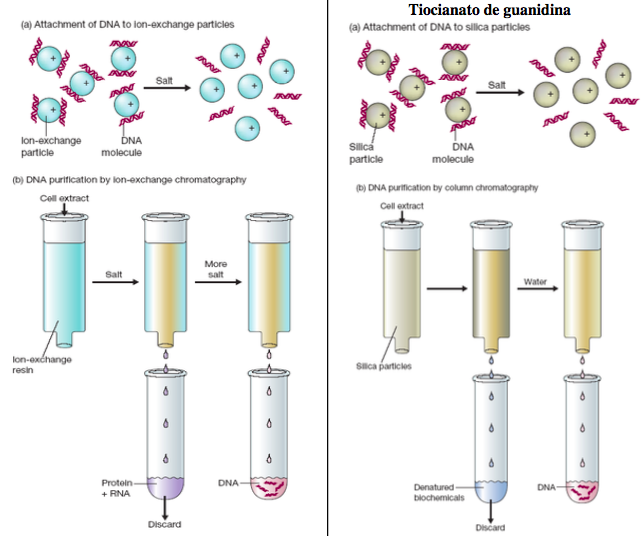
\includegraphics[width=0.8\textwidth]{fig7}
  \caption{Composició parcial en aminoàcids en la cadena $\beta$ humana
    normal i algunes hemoglobines amb cadenes $\beta$ anormals. Altres
    hemoglobines tenen cadenes $\alpha$ anormals.}
  \label{fig:fig7}
\end{figure}

\paragraph{Eritrocitosis} \hfill \\
Alteració en l'afinitat per \ch{O2}. En casos lleus no requereix
farmacologia. L'afinitat és més alta degut a canvis que eviten la unió
de 2,3-difosfoglicerat. Es produeix una hipòxia lleu (augment
d'eritròcits).

\paragraph{Metaglobinèmia} \hfill \\
Alteració en l'afinitat per \ch{O2}. Augmenta la metaglobulina (que és
hemoglobina amb \ch{Fe^3+}). Els eritròcits perden la capacitat de
transportar \ch{O2} i produeix cianosis.

Ens podem trobar:
\begin{itemize}
\item Metaglobinèmia adquirida: Produïda per fàrmacs, oxidants...

\item Metaglobinèmia congènita: Per deficiència de la
  citocrom-b5-reductasa o en presència d'hemoglobina M.
\end{itemize}

Hi ha Hb inestables, com la M que s'oxiden molt fàcilment a
\ch{Fe^3+}. Hi ha 5 tipus d'hemoglobina M, són mutacions al centre de
la unió de la globina al grup hemo. No hi ha afectació en
heterozigosi. L'homozigositat hauria de ser letal però no ho és.

Les manifestacions clíniques són:
\begin{itemize}
\item Cuanosi amb 1.5-2 g d'HbM (malaltia congènita del cor hi ha
  cianosi amb 5g d'Hb desoxigenada/100 mL)
\item Cianosi en el naixement en HbM de cadena alfa.
\item Cianosi als 6 mesos si el defecte està en beta.
\item És convenient fer el diagnòstic per descartar cianosi d'origen
  cardíac, que és molt greu.
\end{itemize}

\subsubsection{Talassèmies}
Són malalties en les que hi ha deficiència de globina, la poca que hi
ha és normal. Les causes són:
\begin{itemize}
\item Deleció gènica
\item Defectes en el processat de RNA
\item Mutacions sense sentit
\item Mutacions stop
\end{itemize}

Les beta talassèmies són més greus perquè només hi ha un locus de
cadena beta-globina.

\paragraph{beta-Talassèmies} \hfill \\
La síntesi de la cadena beta està disminuïda o és nul·la. No està
alterada la síntesi de la cadena alfa.

\begin{itemize}
\item $\beta^0$-talassèmia: No hi ha síntesi de cadena beta de la globina
  (augmenta la $HbA_2$). En homozigots, la HbF i HbA2 està augmentada;
  tenen anpemia microcítica hipocròmica i els eritròcits tenen mida i
  forma normals. Els heterozigots són asimptomàtics.

\item $\beta^+$-talassèmia: Síntesi de la cadena beta disminuïda
  (augmenta la HbA2). Els homozigots tenen els mateixos símptomes que
  l'anterior.

\item $\delta\beta$-talassèmia: Síntesi de la cadena beta i delta de
  globina disminuïdes. La gravetat depèn de si està compensada per una
  síntesi de cadena gamma.

\item $\gamma\delta\beta$-talassèmia: No hi ha síntesi de cadena gamma i
  delta i la cadena beta està disminuïda.
\end{itemize}

\paragraph{$\alpha$-Talassèmies} \hfill \\
Alterada la síntesi de la cadena $\alpha$. Es sinetteitzen en excés les
cadenes gamma (hemoglobina de Bart) i les cadenes beta (hemoglobina
H).

\begin{itemize}
\item alpha^0-Talassèmia: No hi ha síntesi de la cadena alfa de
  globina. La hemoglobina de Bart (tetràmer de delta) representa el 80
  90 \% de la hemoglobina total. És mortal ja que la HbBart no pot
    transportar O2.

  \item alpha^+-Talassèmia: 

  \item Hemoglobinopatia H: 
\end{itemize}

\paragraph*{Estudi bioquímic} \hfill \\
L'estudi de les hemoglobines s'efectua aprofitant la seva mobilitat
electroforètica:
\begin{itemize}
\item Fracció de metahemoglobina: En situacions normals, representa
  menys del 1,5 \% de la hemoglobina en sang. En el cas de la
  metahemoglobinèmia per deficiència de citocrom-b5-reductasa augmenta
  un 10-30 \%.

\item Fracció d'hemoglobina F: En situacions normals representa menys
  de l'1 \% de la hemoglobina en adult.


\end{itemize}


\subsection{Desordres de la síntesi del grup hemo}
La síntesi del grup hemo té lloc un 85\% en eritròcits i un 15\% en el
fetge.

La biosíntesis del grup hemo parteix de succinil-CoA i
glicina. Alteracions en la síntesi del grup hemo produeixen porfíries.

\subsubsection*{Síntesi del grup hemo}
% posar vies i explicar

\subsubsection*{Degradació del grup hemo}
% posar vies i explicar

\subsubsection{Porfíries}
Els principals enzims implicats en les porfíries són:
\begin{itemize}
\item ALA-sintasa: 
Un home de 70 kg té 900 g d'hemoglobina. El bescanvi d'hemoglobina és
de 0,3 g/h (sintetitzats i destruïts).

Classificació de les malalties relacionades amb la hemoglobina:
\begin{itemize}
\item Reaccions de l'hemoglobina
  \begin{itemize}
  \item Metahemoglobinèmia hereditària
  \end{itemize}

\item Síntesi de la globina
  \begin{itemize}
  \item Hemoglobinopaties estructurals
    \begin{itemize}
    \item Anèmies drepanocítiques 
    \item Metahemoglobinèmia congènita
    \item Eritrocitosis (alterada afinitat per O2)
    \end{itemize}
  \item Talassèmies (hemoglobines alterades)
    \begin{itemize}
    \item  $\alpha$-talassèmies
    \item $\beta$-talassèmies
    \end{itemize}
  \end{itemize}

\item Síntesi i degradació del grup hemo
  \begin{itemize}
  \item Porfiries agudes
    \begin{itemize}
    \item Porfíria aguda intermitent 
    \item Coproporfíria hereditària
    \item Porfíria variegata
   \end{itemize}
  \item Porfíries no agudes
    \begin{itemize}
    \item Porfíria eritrohepàtica (eritropoiètica) 
    \item Porfíria eritropoiètica congènita
    \item Porfíria congènita (Intoxicació per plom)
    \end{itemize}
  \end{itemize}

\item Alteracions del metabolisme del ferro
  \begin{itemize}
  \item Anèmia ferropènica (manca de ferro)
    \begin{itemize}
    \item Pèrdua crònica de sang
    \item Ingesta inadequada de ferro
    \end{itemize}
  \item Anèmia sideroblàstica (mala utilització del ferro)
  \item Hemocromatosis (sobrecàrrega de ferro)
  \end{itemize}
\end{itemize}

\subsubsection{Estructura}
Hi ha 6 tipus de globines, que en la seva combinatòria generen els
diferents tipus d'hemoglobina que trobem en humans. Aquests tipus són:
$\alpha$, $\beta$, $\gamma$, $\delta$, $\epsilon$, $\zeta$.

La hemoglobina és un heterotetràmer $\alpha_2\beta_2$ en adults. Presenta
cooperativitat amb l'oxigen. També té al·losterisme amb el
2,3-difosfoglicerat, un intermediari de la glicòlisi que només es
troba en eritròcits. Això facilita l'alliberació d'oxigen als
teixits.

Es sintetitza als reticulòcits (eritròcits immadurs).

La hemoglobina presenta diferents subunitats segons l'estadi de
desenvolupament de l'individu:
\begin{itemize}
\item Adult:
  \begin{itemize}
  \item Hemoglobina A1 ($\alpha_2\beta_2$)
  \item Hemoglobina A2 ($\alpha_2\delta_2$)
  \end{itemize}

\item Fetal: Cadenes $\alpha_2\gamma_2$

\item Embrió:
  \begin{itemize}
  \item Grower I: $\zeta_2\epsilon_2$
  \item Grower II: $\alpha_2\epsilon_2$
  \item Portland: $\zeta_2\gamma_2$
  \end{itemize}
\end{itemize}

Hi ha 2 loci d' $\alpha$-globina al cromosoma 16 i un locus de $\beta$-globina
al cromosoma 11.

\subsection{Trastorns deguts a reaccions de l'hemoglobina}
La carboxihemoglobina presenta menys afinitat per l'hemoglobina.

\begin{figure}[H]
  \centering
  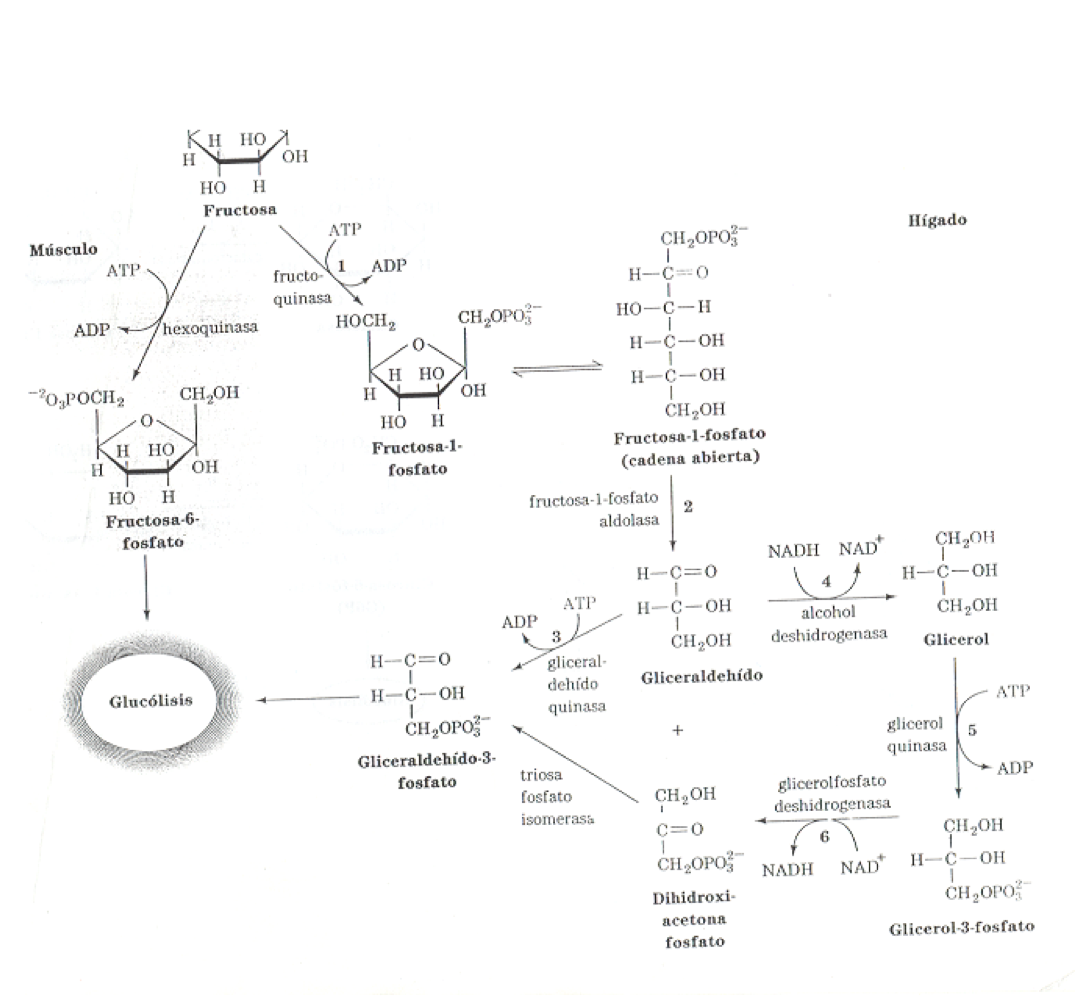
\includegraphics[width=0.5\textwidth]{fig5}
\end{figure}

Molt fàrmacs o agents oxidants poden provocar la formació de
metahemoglobina (amb \ch{Fe3+}), que mitjançant la NADH-metahemoglobina
reductasa la torna a reduir.

\begin{figure}[H]
  \centering
  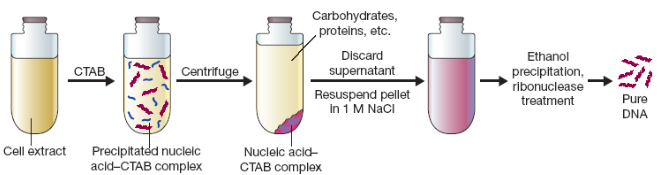
\includegraphics[width=0.5\textwidth]{fig6}
\end{figure}

La metahemoglobinèmia hereditària és una deficiència en NADH-metahemoglobina
reductasa. El Fe del hemo s'oxida en 25 \% a \ch{Fe3+} Es manifesta amb
cianosi (coloració fosca a la pell). Es tracta amb fàrmacs que
redueixin lametahemoglobina. És una malaltia
molt greu.

\subsection{Trastorns a la síntesi de la globina}
\subsubsection{Hemoglobinopaties estructurals}
Les mutacions perjudicials desapareixen, però les altres poden sobreviure
(els heterozigots resisteixen més que els homozigots). Algunes
mutacions són inòcues.

\paragraph{Hemoglobina S. Anèmia drepanocítica} \hfill \\
Es dóna un canvi d'aminoàcid Glu->Val a la cadena beta. És insoluble a baixes pressions
de \ch{O2}. Els glòbuls vermells presenten una morfologia
falciforme. Quan està desoxigenada, la hemoglobina es polimeritza i es
deformen els eritròcits. Els heterozigots  presenten poques vegades símptomes greus

Es va originar a Africa i confereix resistència a la malària. La
presenten un 40 \% de la població africana i un 10\% dels negres
americans.

La Hb pot polimeritzar formant fibres de 3000 \AA{}. Hi ha cicles
successius de forma de falç i normal. La forma de falç es trenca als
capil·lars per falta de flexibilitat. L'anèmia s'agreuja amb oxidants.

Altes concentracions d'HbS d'afinitat baixa per \ch{O2} no donen cap
problema fins l'administració d'un agent oxidant.

L'anèmia és menys severa si és dependent d'HbF. Els pacients tendeixen
a augmentar la proporció d'HbF en l'adult. Els homozigots d'Orient
Mitjà són asimptomàtics ja que tenen un 18\% d'HbF.

El diagnòstic es fa per electroforesi de la hemoglobina o per examen
microscòpic d'un frotis de sang.

Encara no hi ha tractament, encara que hi ha fàrmcs en estudi. La
profilaxi es basa en una bona nutrició i higiene, contra la
malària. En cas d'infecció, s'actua sobre l'agent infecciós. Si es fa
una transfusió quan es dona la primoquina ja que és oxidant i es pot
agreujar l'anèmia.

\paragraph{Hemoglobinopaties inestables} \hfill \\
S'han descrit més de 100 hemoglobinopaties. Es produeix la formació de
cossos d'inclusió intraeritrocítics (cossos de Heinz), que són
precipitacions d'hemoglobina. Consisteix en una sèrie de petites
granulacions que se situen a la perifèria dels hematies. Es produeix
en malalties congènites.

\begin{figure}[H]
  \centering
  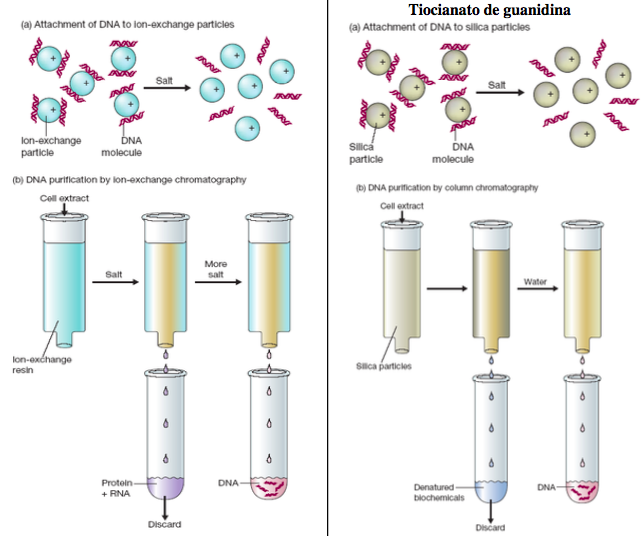
\includegraphics[width=0.8\textwidth]{fig7}
  \caption{Composició parcial en aminoàcids en la cadena $\beta$ humana
    normal i algunes hemoglobines amb cadenes $\beta$ anormals. Altres
    hemoglobines tenen cadenes $\alpha$ anormals.}
  \label{fig:fig7}
\end{figure}

\paragraph{Eritrocitosis} \hfill \\
Alteració en l'afinitat per \ch{O2}. En casos lleus no requereix
farmacologia. L'afinitat és més alta degut a canvis que eviten la unió
de 2,3-difosfoglicerat. Es produeix una hipòxia lleu (augment
d'eritròcits).

\paragraph{Metaglobinèmia} \hfill \\
Alteració en l'afinitat per \ch{O2}. Augmenta la metaglobulina (que és
hemoglobina amb \ch{Fe^3+}). Els eritròcits perden la capacitat de
transportar \ch{O2} i produeix cianosis.

Ens podem trobar:
\begin{itemize}
\item Metaglobinèmia adquirida: Produïda per fàrmacs, oxidants...

\item Metaglobinèmia congènita: Per deficiència de la
  citocrom-b5-reductasa o en presència d'hemoglobina M.
\end{itemize}

Hi ha Hb inestables, com la M que s'oxiden molt fàcilment a
\ch{Fe^3+}. Hi ha 5 tipus d'hemoglobina M, són mutacions al centre de
la unió de la globina al grup hemo. No hi ha afectació en
heterozigosi. L'homozigositat hauria de ser letal però no ho és.

Les manifestacions clíniques són:
\begin{itemize}
\item Cuanosi amb 1.5-2 g d'HbM (malaltia congènita del cor hi ha
  cianosi amb 5g d'Hb desoxigenada/100 mL)
\item Cianosi en el naixement en HbM de cadena alfa.
\item Cianosi als 6 mesos si el defecte està en beta.
\item És convenient fer el diagnòstic per descartar cianosi d'origen
  cardíac, que és molt greu.
\end{itemize}

\subsubsection{Talassèmies}
Són malalties en les que hi ha deficiència de globina, la poca que hi
ha és normal. Les causes són:
\begin{itemize}
\item Deleció gènica
\item Defectes en el processat de RNA
\item Mutacions sense sentit
\item Mutacions stop
\end{itemize}

Les beta talassèmies són més greus perquè només hi ha un locus de
cadena beta-globina.

\paragraph{beta-Talassèmies} \hfill \\
La síntesi de la cadena beta està disminuïda o és nul·la. No està
alterada la síntesi de la cadena alfa.

\begin{itemize}
\item $\beta^0$-talassèmia: No hi ha síntesi de cadena beta de la globina
  (augmenta la $HbA_2$). En homozigots, la HbF i HbA2 està augmentada;
  tenen anpemia microcítica hipocròmica i els eritròcits tenen mida i
  forma normals. Els heterozigots són asimptomàtics.

\item $\beta^+$-talassèmia: Síntesi de la cadena beta disminuïda
  (augmenta la HbA2). Els homozigots tenen els mateixos símptomes que
  l'anterior.

\item $\delta\beta$-talassèmia: Síntesi de la cadena beta i delta de
  globina disminuïdes. La gravetat depèn de si està compensada per una
  síntesi de cadena gamma.

\item $\gamma\delta\beta$-talassèmia: No hi ha síntesi de cadena gamma i
  delta i la cadena beta està disminuïda.
\end{itemize}

\paragraph{$\alpha$-Talassèmies} \hfill \\
Alterada la síntesi de la cadena $\alpha$. Es sinetteitzen en excés les
cadenes gamma (hemoglobina de Bart) i les cadenes beta (hemoglobina
H).

\begin{itemize}
\item alpha^0-Talassèmia: No hi ha síntesi de la cadena alfa de
  globina. La hemoglobina de Bart (tetràmer de delta) representa el 80
  90 \% de la hemoglobina total. És mortal ja que la HbBart no pot
    transportar O2.

  \item alpha^+-Talassèmia: 

  \item Hemoglobinopatia H: 
\end{itemize}

\paragraph*{Estudi bioquímic} \hfill \\
L'estudi de les hemoglobines s'efectua aprofitant la seva mobilitat
electroforètica:
\begin{itemize}
\item Fracció de metahemoglobina: En situacions normals, representa
  menys del 1,5 \% de la hemoglobina en sang. En el cas de la
  metahemoglobinèmia per deficiència de citocrom-b5-reductasa augmenta
  un 10-30 \%.

\item Fracció d'hemoglobina F: En situacions normals representa menys
  de l'1 \% de la hemoglobina en adult.


\end{itemize}


\subsection{Desordres de la síntesi del grup hemo}
La síntesi del grup hemo té lloc un 85\% en eritròcits i un 15\% en el
fetge.

La biosíntesis del grup hemo parteix de succinil-CoA i
glicina. Alteracions en la síntesi del grup hemo produeixen porfíries.

\subsubsection*{Síntesi del grup hemo}
% posar vies i explicar

\subsubsection*{Degradació del grup hemo}
% posar vies i explicar

\subsubsection{Porfíries}
Els principals enzims implicats en les porfíries són:
\begin{itemize}
\item \textbf{ALA-sintasa:} Activitat baixa, però influïble per medicaments i esteroides. Presenta retroinhibició pel grup hemo i per l’hemina (hemo-Fe(III)).

\item \textbf{Uroporfirinògen sintasa:} Control secundari.
\end{itemize}

Hi ha 2 tipus de porfírires:
\begin{enumerate}
\item Porfíries agudes:

\item Porfíries no agudes:
\end{enumerate}

\paragraph{Porfírires agudes} \hfill \\

\subparagraph{Porfíria aguda intermitent}  \hfill \\
És la més freqüent. S'hereta amb caràcter autosòmic dominant.
Es tracta d'una deficiència en hidroximetilbilà sintasa (E.C. 4.3.1.89.). Afecta a 3 dones per cada 2 homes.

Els símptomes són dolor abdominal espasmòdic, vòmits, estrenyiment, febre, leucocitosi, hematúria.

L'anàlisi bioquímic es basa en ALA i porfobilinogen.

\subparagraph{Coproporfíria hereditària} \hfill \\
S'hereta amb caràcter autosòmic dominant.
És una deficiència en coproporfirinògen-oxidasa (E.C. 1.3.3.3.). Els pacients són assimptomàtics o presenten lleus símptomes neurològics, abdominals o psiquiàtrics.

Hi ha una excreció constant de coproporfirina III en femta. També hi ha una excreció de forma intermitent de coproporfirina, aàcid aminolevulínic i porfobilinògen en orina.

S’atribueix a un bloqueig del pas coproporfirina III $\rightarrow$ protoporfirina, una inducció de ALA-sintetasa o les dos coses a la vegada.

\subparagraph{Porfíria variegata} \hfill \\
Deficiència en protoporfirinògen-oxidasa (E.C. 1.3.3.4.). Afecta de manera igual a homes i dones. Predomina entre la població blanca d’Africa. Apareix entre la tercera i quarta dècada de la vida.

Símptomes: similars als de la porfíria aguda intermitent, amb lessions cutànies. 

\paragraph{Porfíries no agudes} \hfill \\

\subparagraph{Porfíria hepàtica-cutània (hepatocutània)}  \hfill \\
Casos familiars rars. És un grup de porfiries adquirides Símptomes: lessions cutànies
Associada a malaltia hepàtica (estímul alcohòlic, tractament amb estrògens, ingesta de hexaclorobenzè).

Excreció elevada de uroporfirina en orina. Valors normals de PBG i ALA

\subparagraph{Protoporfíria eritrohepàtica (eritropoiètica)} \hfill \\
S’hereda amb caràcter autosòmic dominant
Afecta a eritròcits i a fetge
Lleu fotosensibilitat cutània
Apareix en primers anys de la vida o etapa adulta
Elevada quantitat de protoporfirina a la circulació
Nivells fecals elevats de protoporfirina i coproporfirina (fluorescència de la femta)
Activitat excessiva de ALA sintasa

\subparagraph{Protoporfíria eritropoiética congènita} \hfill \\
S’hereda amb caràcter autosòmic recessiu
Poc freqüent, es manifesta just després del part
Base bioquímica de la llegenda del ``home-llop''
Orina color vermell (excreció de coproporfirina i uroporfirina), eritrodòncia (dipòsits vermells fluorescents a les dents), anèmia hemolítica, intensa fotosensibilitat cutània (úlceres i cicatrius), aparició de pèls fins en cara i extremitats.
Esplenomegàlia, anèmia hemolítica, mort precoç
Defecte enzimàtic de la uroporfininògen III cosintetasa. Augment de la ALA-sintetasa

\subparagraph{Intoxicació per plom} \hfill \\
 Símptomes per intoxicació per plom (dolors abdominals, estrenyiment,...) es deuen a inhibició d’algun dels enzims de síntesi de hemo.
Disminució de ALA-deshidratasa, ferroquelatasa i oxidasa del coproporfirinògen
Anàlisi al laboratori: ALA  i coproporfirines en orina.

\subsubsection*{Anàlisi de la porfirina}
Totes les porfirines tenen un espectre UV pròxim – visible. Es veu una intensa banda a 400 nm (Banda de Soret) que emet fluorescència vermella. Es poden quantificar valors de $2\cdot 10^4 \mu mol/L$. La solubilitat disminueix en reduir grups hidroxil i carboxils:
\begin{itemize}
\item PBS i uroporfirina: s’excreten en orina
\item Protoporfirina: via bilis   s’excreta en femta
\item Coproporfirina s’excreta en orina com a coproporfirinògen
\end{itemize}

La determinació d'ALA i PBG es fa pel mètode de Watson (1941). El PBG es condensa amb p-dimetil-aminobenzaldehid en àcid clorhídric (reactiu d’Ehrlich) i forma un complexe magenta.

Les porfirines es determinen amb una extracció amb dissolvent orgànic (àcid acètic, acetat d’etil), una extracció de HCl o bé per determinació espectrefotomètrica o fluorimètrica.

La determinació d'ALA-deshidratasa és molt útil en intoxicacions per plom (a més de plumbèmia, coproporfirines i ALA). El mètode de Bonsignore mesura el PBG produit (el PBG es transforma a porfirina durant l’assaig). El mètode de Tomokumi mesura l'ALA consumida.

\subsection{Alteracions del metabolisme del ferro}
L'anèmia és una condició patològica en què la concentració d'hemoglobina és molt baixa, i hi ha una pèrdua de la capacitat del transport d'oxigen.

% posar taula valors normals

Els eritròcits són discs bicòncaus de 2 micres d'amplada i 7 micres de diàmetres. Un 66\% és aigua i un 33\% és Hb. Tenen una vida mitjana de 120 dies. Moren fagocitats a la melsa, fetge i medul.la òsea
Funció principal: donar suport a la hemoglobina per transportar \ch{O2} i \ch{CO2}. Es transporta el 20\% del \{CO2} produit als teixits   contribueixen en la capacitat tamponadora de la sang.

La eritropoiesi és el procés de producció d'eritròcits. Regulat per la hormona eritropoietina (regulada per la quantitat de O2 que arriba als teixits).

Hi ha 2 tipus d'anèmies:
\begin{itemize}
\item Anèmies arregeneratives per fallida a la eritropoiesis:
  \begin{enumerate}
  \item Fallida qualitativa: lesió de la cèl.lula mare pluripotent
    \begin{enumerate}
    \item Aplàsia medular
    \item Aplàsia medicamentosa
    \item Fibrosis medular
    \item Anèmia mieloptísica per invasió medular (neoplasies, mielomes, etc.)
    \item Mecanisme autoimmune
    \end{enumerate}
  \item Fallida quantitativa: alteració de la maduració eritroblàstica
    \begin{enumerate}
    \item Carencials (per dèficit de cianocobalamina, folats o ferro).
    \item Diseritropoyètiques (bloqueig del ferro, talasèmies i bloqueig de la síntesi del grup hemo)
    \item Mixtes, per neoplàsies, cirrosis, infeccions o lesions renals
    \end{enumerate}
  \end{enumerate}

\item Anèmies regeneratives:
  \begin{enumerate}
  \item Per pèrdua d’eritròcits: hemorràgiques
    
  \item Per augment de la destrucció dels eritròcits: hemolítiques
    \begin{enumerate}
    \item Anèmies hemolítiques congèniques:
      \begin{enumerate}
      \item Anomalies de la membrana (esferocitosis, eliptocitosis, xerocitosis, etc.)
      \item Alteracions enzimàtiques (dèficit de glucosa-6-P deshidrogenasa, dèficit de piruvat kinasa, etc.)
      \item Hemoglobinopaties (talasèmies i hemoglobinopaties estructurals)
      \end{enumerate}
    \item Anèmies hemolítiques adquirides:
      \begin{enumerate}
      \item Autoimmunes i postransfusionals
      \item Causes mecàniques (anèmia microangiopàtica)
      \item Causes infeccioses o químiques
      \item Causes desconegudes (hemoglobinúria paroxísticanocturna)
      \end{enumerate}
    \end{enumerate}
  \item Per recuperació d’una anèmia carencial tractada
  \end{enumerate}
\end{itemize}

\subsubsection{Anèmies megaloblàstiques}
Degudes al dèficit de cianocobalamina o folat, que intervenen en la síntesi de DNA que estarà disminuïda. Hi ha una alteració de l'eritropoiesi (asincronia madurativa entre nucli i citoplasma de cèl.lules precursores de l’eritròcit). L'eritropoiesi és ineficaç.

Les causes principals d'anèmies megaloblàstiques són:
\begin{itemize}
\item Deficiència de cobalamina
  \begin{itemize}
  \item Dèficit en l’alimentació (vegetarians estrictes)
    
  \item Déficit de secreció del factor intrínsec (Anèmia perniciosa):
    \begin{itemize}
    \item per la destrucció de mucosa gàstrica o postgastrectomia
      
    \item per l’existència d’un factor intrínsec biològicament inactiu
      
    \item per l’existència d’anticossos contra el factor intrínsec
    \end{itemize}
    
  \item Alteració del budell prim: Malabosrció o parasitació per Dibothriocephalus latus.

  \item Deficiència de transcobalamina
  \item Augment de les necessitats de cianocobalamines: Embaràs o augment de la prooliferació cel·lular.
  \end{itemize}
\item Deficiència de folat
  \begin{itemize}
  \item Dèficit en la dieta
    
  \item Malabsorció
    
  \item Interferències farmacològiques en la seva metabolització
  \item Augment de les necessitats: Embaràs o augment de la prooliferació cel·lular.
  \end{itemize}
\end{itemize}

\paragraph{Anàlisi bioquímic}
Aiugmenta el Fe oxidat ja que no es pot utilitzar de forma adequada pel transport d'oxigen.

Pot augmentar el folat i la B12 en plasma si s'ingereix però hi ha una malabsorció.

\paragraph{Prova de Schilling}
Estudia la causa de la disminució de cobalamina per diferenciar entre anèmia perniciosa i malabsorció. Es basa en l'administració al pacient de 2 càpsules per via ora:
\begin{itemize}
\item 57Co-cianocobalamina + factor intrínsec
  
\item 58Co-cianocobalamina sense factor intrínsec
\end{itemize}

Després d'administra cianocobalamina per via intramuscular. Aquesta injecció satura el transportador sanguini (transcobalamina II) i obliga la secreció via orina de la cobalamina ingerida. Després es mesura la radioactivitat en orina 24 h després de la injecció.

\subsubsection{Anèmies hemolítiques}

\subsubsection{Anèmia ferropènica}


\subsubsection{Anèmia sideroblàstica}


\subsubsection{Hemocromatosis}


\subsection{Casos clínics}

\begin{enumerate}[\bf 1)]
\item 
\end{enumerate}